% !TEX root = ../thesis.tex
\section{Analýza dat a první modely}
\label{chap:experiments:analysis}

Rozpoznávání řeči se věnuje nemalé usílí již od 50. let 2O. století a v současné době nikoho nepřekvapí téměř bezchybně fungující obecný rozpoznávač v mobilních zařízeních. Pro obecné systémy dokonce existují korpusy s desítkami či stovkami a více hodin promluv, které je možné využít při vytváření těchto systémů.

Tyto korpusy však obsahují ve většině případů pouze \uv{standardní}\footnote{Slovením spojením \uv{standardní řeč} je myšlena řeč neobsahující vyrazné řečové vady, případně jiné formy produkce a často v nepřílíš akusticky náročném prostředí.} řeč. Pokud je snaha vytvořit nebo ověřit funkčnost systému za specifických podmínek (ať už se jedná o rušné prostředí či speciální typy promluv), tak je nezbytné získat potřebná data.

\subsection{Vytvoření korpusu EL promluv}
\label{chap:experiments:analysis:corpus}

Na začátku byla idea o pomoci skupině lidí mající problémy s přirozenou řečí. Vůbec prvním předpokladem, na cestě k úspěšnému dosažení vůbec nějakého cíle, jsou data. Jelikož se jedná o velmi spefická data, tak je potřeba zajistit co možná největší množství kvalitních\footnote{Kvalitou je myšlena věrnost dat dané doméně, dále se mluví o přesnosti ve smyslu bezchybnosti přepisů.} a přesných dat.

V části \ref{sec:cause:desease} bylo zmíněno, že ročně se objevý více než 100 nových případů trvalé ztrázy hlasu ročně. Zaroveň bylo řečeno \cite{Skvrnakova2010}, že více rizikovými osobami jsou starší lidé, kteří intenzivně kouří a konzumují alkohol. Přesto je patrný trend snižujícího se věku pacientů a s tím souvisejícím nárůstem případů ztráty hlasu. Přičteme-li již zmíněný psychologický aspekt jeho ztráty, tak je zřejmé, jak komplikované je získat ke spolupráci i jen jednoho řečníka ochotného podstoupit naročné\footnote{I pro zdravého člověka je někdy někalikahodinové nahrávání vysilující. Pro jedince po TL to je z mnoha důvodů ještě řádově náročnější.} nahrávání.

Při libovolné práci s pacienty po TL, dřív nebo později dojde k určité formě spolupráce s oddělením ORL, které má nastarosti péči o tyto pacienty. V našem připadě nejprve s ORL klinikou při Fakultní nemocnici v Plzni a poté i s ORL klinikou Fakultní nemocnice v Motole. S jejich pomocí jsme získali ke spolupráci jednoho řečníka. Konkrétně se jedná o dámu v duchodovém věku, která podstoupila TL před více než 15 lety. Po překonání ostychu\footnote{Podle jejích vlastních slov nebyla schopna několik let po operaci ani zvednout nečekaný telefonní hovor, natož mluvit na veřejnosti.} se byla schopna naplno vrátit do běžného života a dokonce v určité formě opět přednášet o stomatologii na Lekařské fakultě v Plzni Univerzity Karlovy.

S její pomocí jsem, v 1. etapě nahrávání, byli schopni pořídit přes 10 hodin promluv, viz tab. \ref{tab:experiments:analysis:recording}. Nahrávání probíhala v relativně spartánských podmínkách za plného běžného provozu katedry. Přesto získaná data neosahují žádný nežadoucí ruch, kromě toho produkovaného samotným EL.

Nahravací aparatůra sestávala z miniaturního profesionálního mikrofonu (DPA d:screet 4061-FM), zesilovačem (DPA MMA6000), externí zvukovou kartou a běžného notebooku. Mikrofon byl pomocí bezpolštářkové náplasti přilepen poblíž pravého koutku úst, abychom zaznamenaná řeč měla co možná nejvyšší kvalitu.

Celé nahrávání bylo v 1. etapě rozděleno do 14 samostatných sezení a probíhalo od prosince roku 2010 do května roku 2011. Každé sezení trvalo přibližně dvě hodiny během kterých se podařilo získat necelou hodinu akustických dat. Samotné nahrávání se sestávalo z 10 - 20 minutového úseku pořizování nahrávky a přibližně 10 minut dlouhého odpočinku. Ten byl nezbytný hlavně z důvodu únavy řečníka.

Ještě před samotným nahrávánám byly pečlivě vybrány a vytvořeny 2 sady vět:

\begin{enumerate}
  \item sada obsahující všechny možné české fonémy - \textit{40 vět}.
  \item sada obsahující věty s reálnou četností fonémů - \textit{5000 vět} \cite{Radova2000}.
\end{enumerate}

\noindent Pořízené nahrávky vždy odpovídají 10 - 20 minutovému úseku nepřerušovaného nahrávání a soubory tak vždy obsahují několik vět. Ty jsou od sebe odděleny minimálně 5 sekundovým úsekem ticha. Nahrávky dále mouhou obsahovat opakování chybně vyslovené věty, přeřeknutí, kýchnutí a další neřečové události. Z tohoto důvodu bylo nezbytné pořízené nahrávky anotovat, přestože byly pořízené na základě připravené sady vět.

Ještě před samotným anotováním byly nahrávky, podle úseků s tichem, rozsekány na menší části. V tomto případě úplně dobře nefungovali\footnote{Problémem byl zvuk EL, se kterým nebylo při návrhu VAD počítáno.} standardně používané sofistikovanější metody pro voice activity detection (angl. zkratka VAD), a proto bylo využito principu energie. Pro každou nahrávku obsahující více vět se pomocí vzorce

\begin{equation}
  \label{eq:experiments:analysis:energy}
  E_{RMS}(n) = \sqrt{\frac{1}{N} \sum_{n=1}^{N} \left| x(n) \right|^2},
\end{equation}

\noindent kde $N$ představuje počet vzorků v nahrávce a $x(n)$ představuje pravoúhlé okénko vzorku $n$. Pro tento případ se ukázalo jako vhodnější volit root-mean-square energy ($E_{RMS}$) a empericky se ukázalo, že vhodná délka okénka je v rozmezí $10 - 100$ ms. Na obr. \ref{fig:experiments:analysis:el_speech} je zobrazena podoba audio signálu a spektrogram promluvy \textit{\uv{Akcie Komerční banky}}. Zároveň je zde vypočtené hodnoty energie a celková průměrná energie. Tyto hodntoty slouží pro určení míst kde začíná a končí věta. Na začátku a konci každé věty je dobré mít minimálně $0.5$ s ticha. Tím pádem, pokud energie nějakého úseku $x$ je $E_{RMS}(x) < avg(E_{RMS})$ a zároveň délka tohoto úseku $dur(x) \geq 1\ [s]$, tak nahrávku můžeme v tomto úseku rozdělit.

\begin{figure}[hbpt]
  \centering
  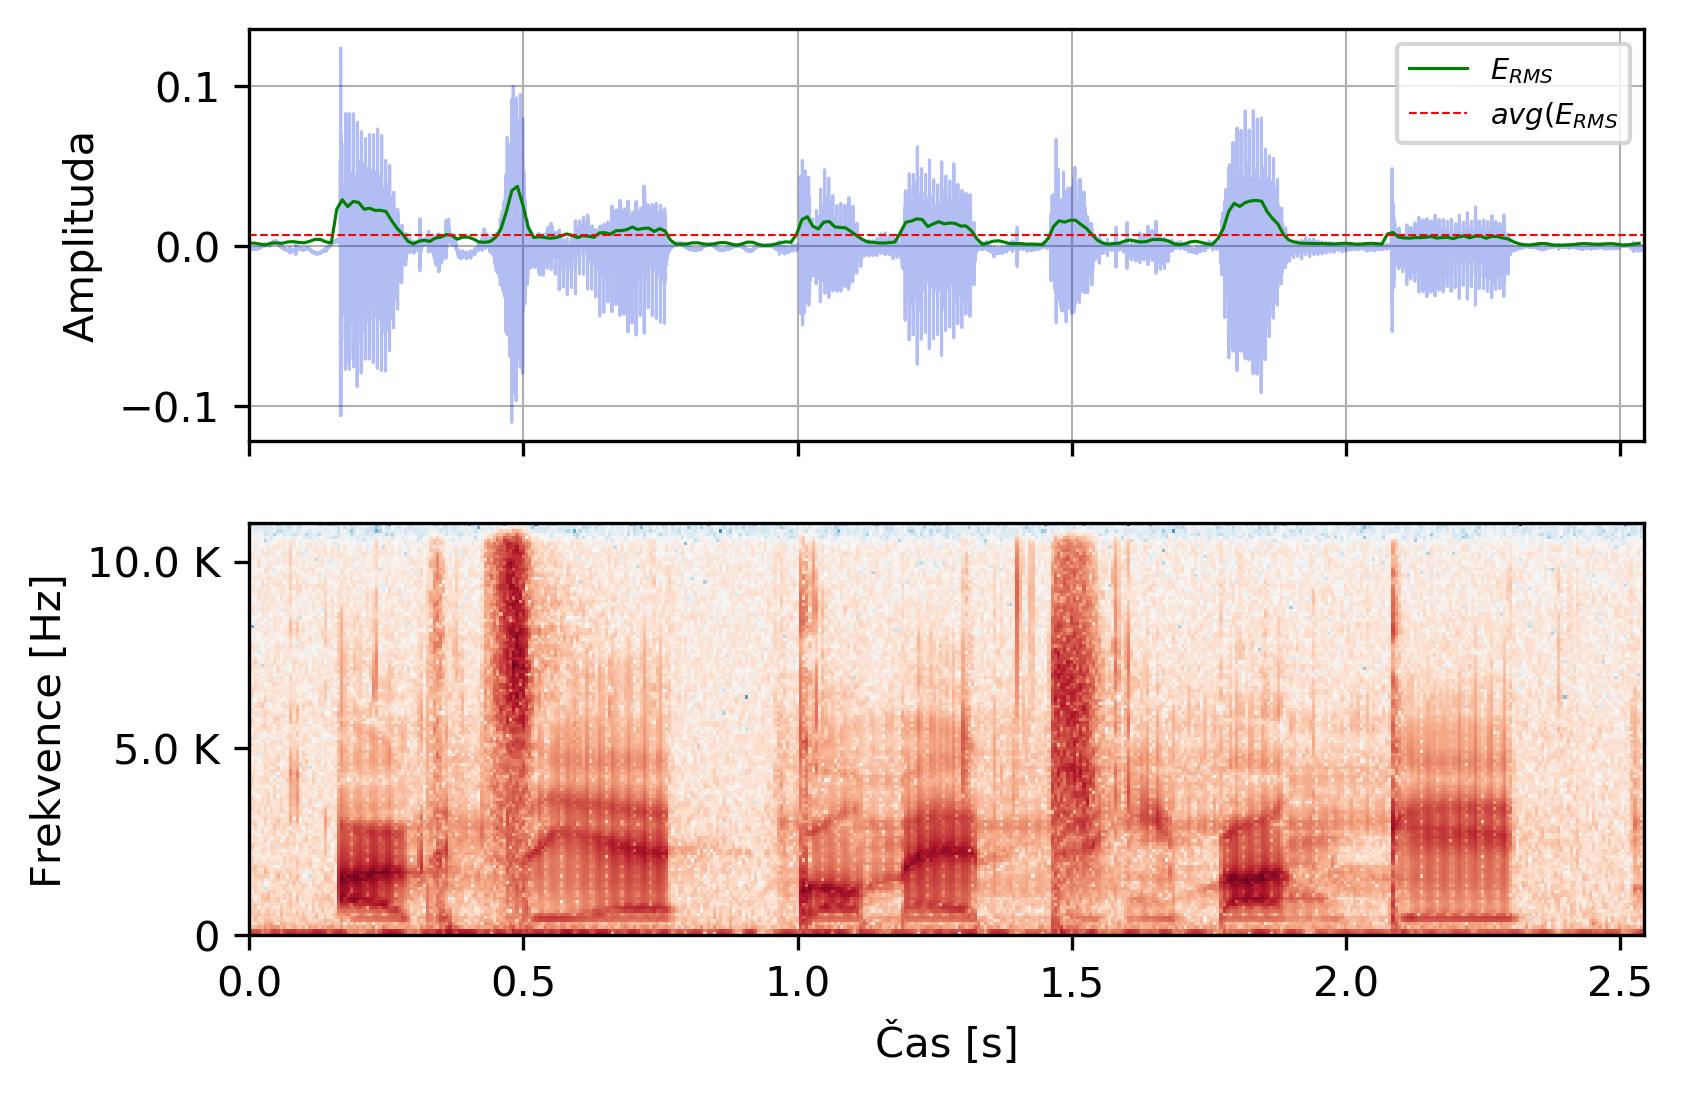
\includegraphics[width=0.9\textwidth]{./ch4-experiments/img/energy_spec_el.png}
  \caption{Průběh a spektrogram promluvy a vyznačenou energií EL promluvy.}
  \label{fig:experiments:analysis:el_speech}
\end{figure}

Samozřejmě pokud řečník v průbehu věty z libovolného důvodu udělal větší pauzu než $1$ s, tak tato věta byla rozdělena. Jelikož jsou výsledné kratší useky promluv následně anotovány, tak to nepředstavuje problém. Pro budoucí zpracování není podstatné zda promluva je opravdu celá věta, ale to jestli je tento úsek správně přepsán. Fakt, že některé věty jsou rozděleny je důvodem proč v tab. \ref{tab:experiments:analysis:recording} více souborů než vět.

K anotaci posloužil interní nástroj určený k tomuto účelu a podíleli se na něm celkem 3 anotátoři z řad studentů, kteří si vzájemně kontrolovali své anotace. Ačkoli bylo potřeba anotovat relativně malé množství dat (cca 10 hodin audio záznamu), tak anotace zabrala přibližně 2 měsice. Hlavním důvodem byla relativně dlouhá doba, po kterou se anotátoři adaptovali na specificka EL řeči. Problémem bylo to, že nejprve nebyli vůbec schopni poruzumnět obsahu promluvy a tím pádem jej správně přepsat.

Pokud je pro produkci řeči použit elektrolarynx, tak vedlejším produktem je nezanedbatelný ruch způsobený samotným zařízením \ref{sub:cause:treatment:foniatric}. Přeci jen jeho jedinout funkcí je vybudit vzduch v dutině ústní a tím umožnit produkci slyšitelné řeči. Z tohoto důvodu byly v průběhu anotace ignorovány v podstatě všechny skupiny neřečových událostí, protože vetšinu obsahu nahrávek by bylo nezbytné anotovat jako, že obsahují šum.

Výsledný korpus tedy představuje $5040$ unikátních vět rozdělených do $6385$ souborů (viz tab. \ref{tab:experiments:analysis:recording}), které v průměru obsahují $7$ slov o průmerné délce $5$ znaků. Tento korpus slouží jako základ pro všechny budoucí experimenty.

\begin{table}[htpb]
  \centering
  \def\arraystretch{1.5}
  \pgfplotstabletypeset[
    col sep=comma,
    string type,
    columns/phase/.style={column name=Nahrávání, column type={|l}},
    columns/length/.style={column name=Délka \textit{[HH:MM:SS]}, column type={|r}},
    columns/sentences/.style={column name=Počet vět, column type={|r}},
    columns/files/.style={column name=Počet souborů, column type={|r|}},
    every head row/.style={after row=\hline, before row=\hline},
    every last row/.style={after row=\hline},
  ]{./ch4-experiments/tabs/02-recording1-stats.csv}
  \caption{Informace o korpusu nahrávek z 1. etapy nahravání.}
  \label{tab:experiments:analysis:recording}
\end{table}

\subsection{Analýza získaných dat}
\label{chap:experiments:analysis:data}

Po dokončení anotace obsahuje korpus přes 10 hodin akustických záznamů promluv a více či méně přesných přepisů\footnote{I přes nemalou snahu a několikastupňovou kontrolu, je téměř jisté, že by nebylo obtížné najít přepis, který obsahuje chybu například ve formě překlepu.}. Když jsou k dispozici data je možné se podívat na specifika EL řeči a případně porovnat se zdravým řečníkem.

Pro potřeby porovnání byl použit začátek promluvy \textit{\uv{Akcie Komerční banky...}}. Tuta promluva je součástí standardní množiny vět používaných při vytváření řečových korpusů na KKY při ZČU. Tím pádem je k dispozici v relativně velkém množství příkladů pro zdravé řečníky a také je součástí korpusu EL řeči.

Na obr. \ref{fig:experiments:analysis:el_speech} a \ref{fig:experiments:analysis:normal_speech} je zobrazen průběh signálu a spektrogram vybrané promluvy. Už na první pohled je možné zaznamenat určité rozdíly. Prvním takovým je délka promluvy, v případě zdravého řečníka je o celou 1 vteřinu kratší než v případě EL řeči. Tempo řeči je samozřejmě velmi individuální, ale z principu je EL řeč pomalejší. Z průbehu signálu na obr. \ref{fig:experiments:analysis:el_speech} je patrné, že řečník dělá výraznější pauzy mezi jednotlivými slovy promluvy. To může být způsobené například potřebou naplnit jícen vzduchem. Po TL je dýchání realizováno přes tracheu a pokud nebyl voperován shunt (více v \ref{sub:cause:treatment:tracheo}), tak je trvale oddělen hrtan a hltan. Přesto, pro produkci některých neznělých fonémů je potřeba exhalovat vzduch z dutiny ústní. Zkušený EL řečník to dělá naprosto automaticky, nicméně \uv{polykání} vzduchu zabere nějaký čas. Nevyhnutelným důsledkem je pak velmi častý výskyt samovolného říhání v průběhu promluvy\footnote{Fakt, že je říhání jako neřečová událost běžnou součástí téměř každé promluvy, vedl k ignorování těchto událostí během anotace.}.

\begin{figure}[hbpt]
  \centering
  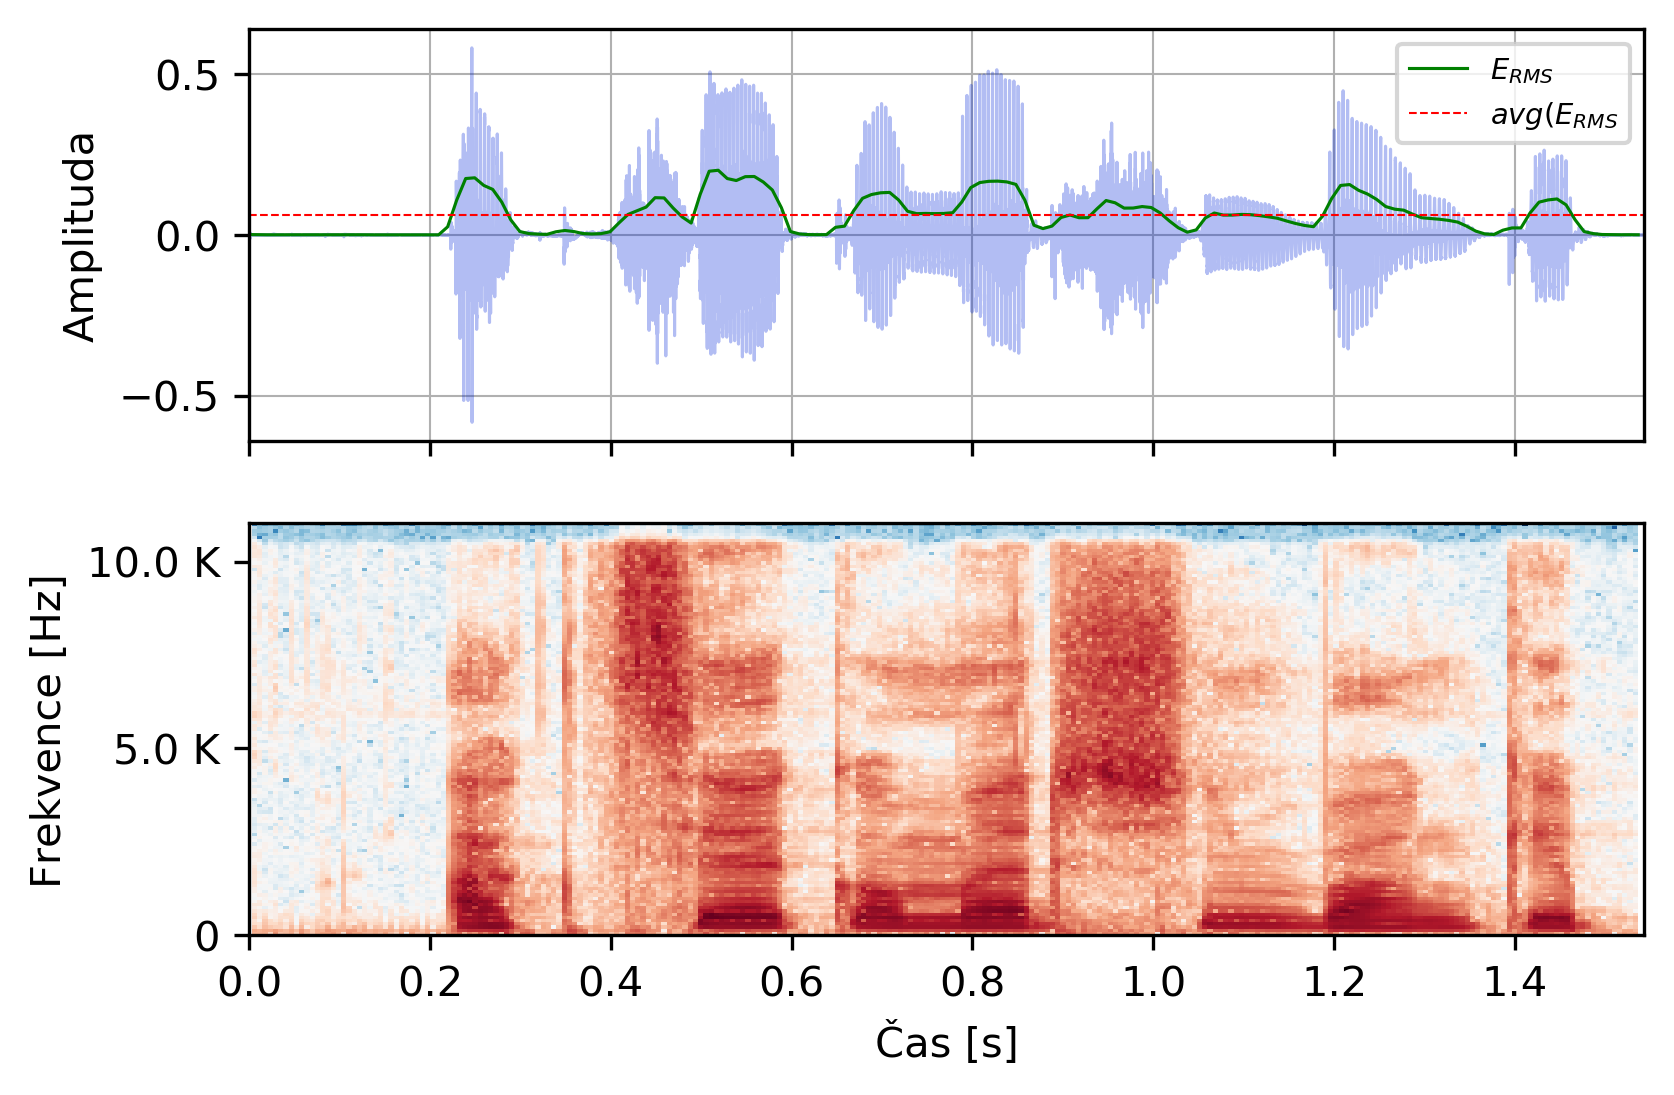
\includegraphics[width=0.9\textwidth]{./ch4-experiments/img/energy_spec_normal.png}
  \caption{Průběh a spektrogram promluvy a vyznačenou energií promluvy.}
  \label{fig:experiments:analysis:normal_speech}
\end{figure}

Dalším důvodem může být je nutnost správné artikulace. Při používání EL je to nezbytné, aby bylo produkované řeči alespoň trochu dobře rozumnět. A pokud se dobře artikuluje, tak není snadné mluvit rychle. Při nahrávání bylo také velmmi běžné, že v průběhu promluvy řečník udělal pauzu, aby mohl lépe umístit EL, protože jeho umístění má velký vliv na kvalitu produkované řeči. Nicméně je třeba říci, že tempo není a priory pro ASR systémy problém, protože různá délka fonémů je v relativně snadno modelována, např. v \textit{HMM} přechodem ze stavu do stejného stavu.

Dalším způsobem jak ukázat rozdíly mezi promluvou zdravého řečníka a řečníka s EL je srovnání ve frekvenční oblasti. Pro větší názornost jsou na obr. \ref{fig:experiments:analysis:spectrogram} vedle sebe zobrazeno spektrum ukázková promluva zdravého řečníka (\ref{fig:experiments:analysis:spectrogram:normal}) a toho s EL (\ref{fig:experiments:analysis:spectrogram:el}). Obsah obou promluv je identický a přesto jsou obě spektra odlišná.

Prvním markantním rozdílem je mnohem větší zastoupení šumu v úsecích \uv{ticha} na obr. \ref{fig:experiments:analysis:spectrogram:el}. To je nepochyně způsobnemo samotným EL, který řečník nevypíná mezi jednotlivými slovy. Na obr. \ref{fig:experiments:analysis:el_speech} je to také zřetelně patrný, zejména na průběhu energie, šum zejména před prvním a druhým slovem promluvy. Zajímavá je přítomnost šumu v célém frekvenčním spektru, přestože EL produkuje konstantní buzení. Toto buzení je ve spektru, na obr. \ref{fig:experiments:analysis:spectrogram:el}, viditelná jako výrazná souvislá linie v nízkých frekvencích. Přitomnost šumu ve vyšších frekvencích je způsobena umístěním mikrofonu, který je nalepen na pokožku a tím pádem snímá namodulované vibrace, přenášené měkkou tkání. Tento fakt se potvrdil v dalších etapách nahrávání (viz část \ref{chap:experiments:normalization:corpus}), kde je použit studiový mikrofon vzdálený od úst minimálně 15 cm a tyto vibrace již nezaznamenává. Nicméně z pohledu použitelnosti nějakého budoucího systému je nezbytné počítat i se situací, kdy mikrofon bude zaznamenávat i vibrace přenášené tkání.

Dalším markantním rozdílem je absence vyšších frekvencí u většiny produkovaných fonémů. Vyjímku tvoří afrikáty $/c/$ a $/\check{c}/$, u kterých jsou hlasivky (u zdravého jedince) v klidu a vznikají uvolněním nahromaděného vzduchu v dutině ústní\footnote{Nahromadění vzduchu je realizováno přitisknutím jazyka k přední/zadní části horního patra.} \cite{Psutka2006}. V tomto případě není, u řečníka po TL, principiálně tento mechanizmus produkce těchto fonému ovlivněn. Problémem teoreticky může být zdroj vzduchu, jelikož jej z plic není možné dostat do dutiny ústní, ale jak už bylo zmíněno (a spektrogram to potvrzuje) zkušený uživatel EL se dokáže adaptovat.

Absence vyšších frekcencí se dá vysvětlit použitím EL, kde samotný EL má vždy konstantní frekvenci buzení a dále tím, že nedochází k modulaci v ve všech dutinách vokálního traktu. Nicméně nejdůležitější složky, zajišťující srozumitelnost, se vyskytují ve frekvenčním pásmu od 1 kHz do 3 kHz. Vyšší frekvence se a priory podílejí na zabarvení hlasu.

\begin{figure}[htpb]
  \centering
  \begin{subfigure}[b]{0.4\textwidth}
    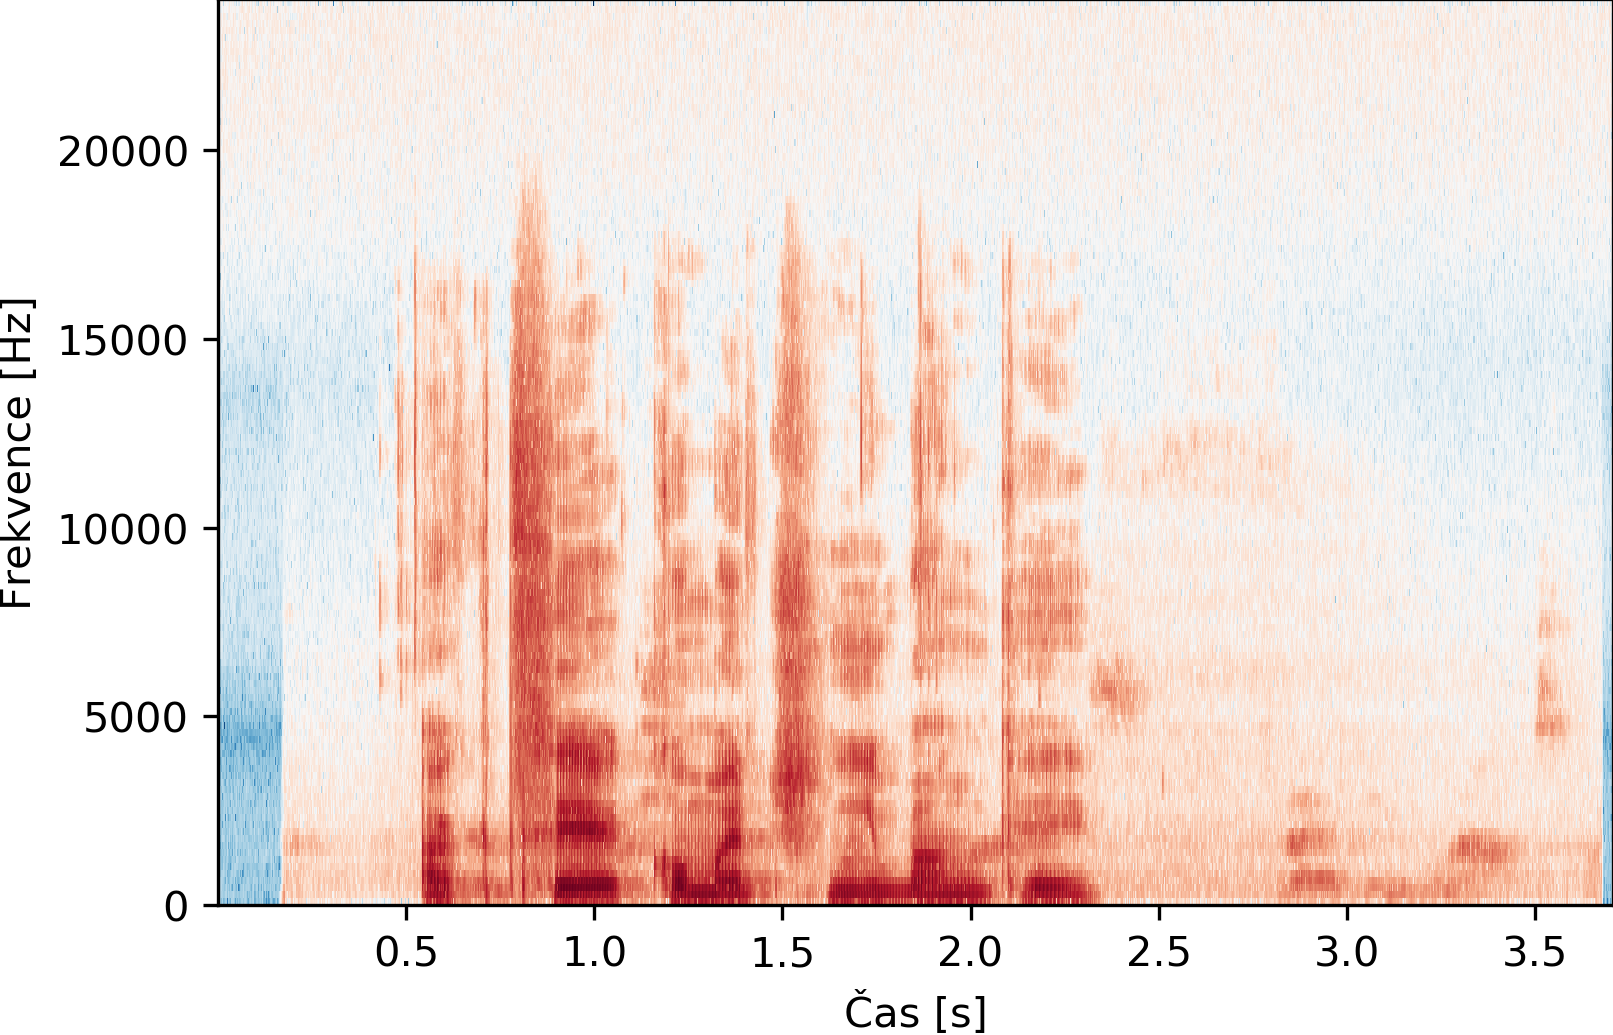
\includegraphics[width=\textwidth]{./ch4-experiments/img/spectrogram_normal.png}
    \caption{Zdravý řečník}
    \label{fig:experiments:analysis:spectrogram:normal}
  \end{subfigure}
  %
  \begin{subfigure}[b]{0.4\textwidth}
    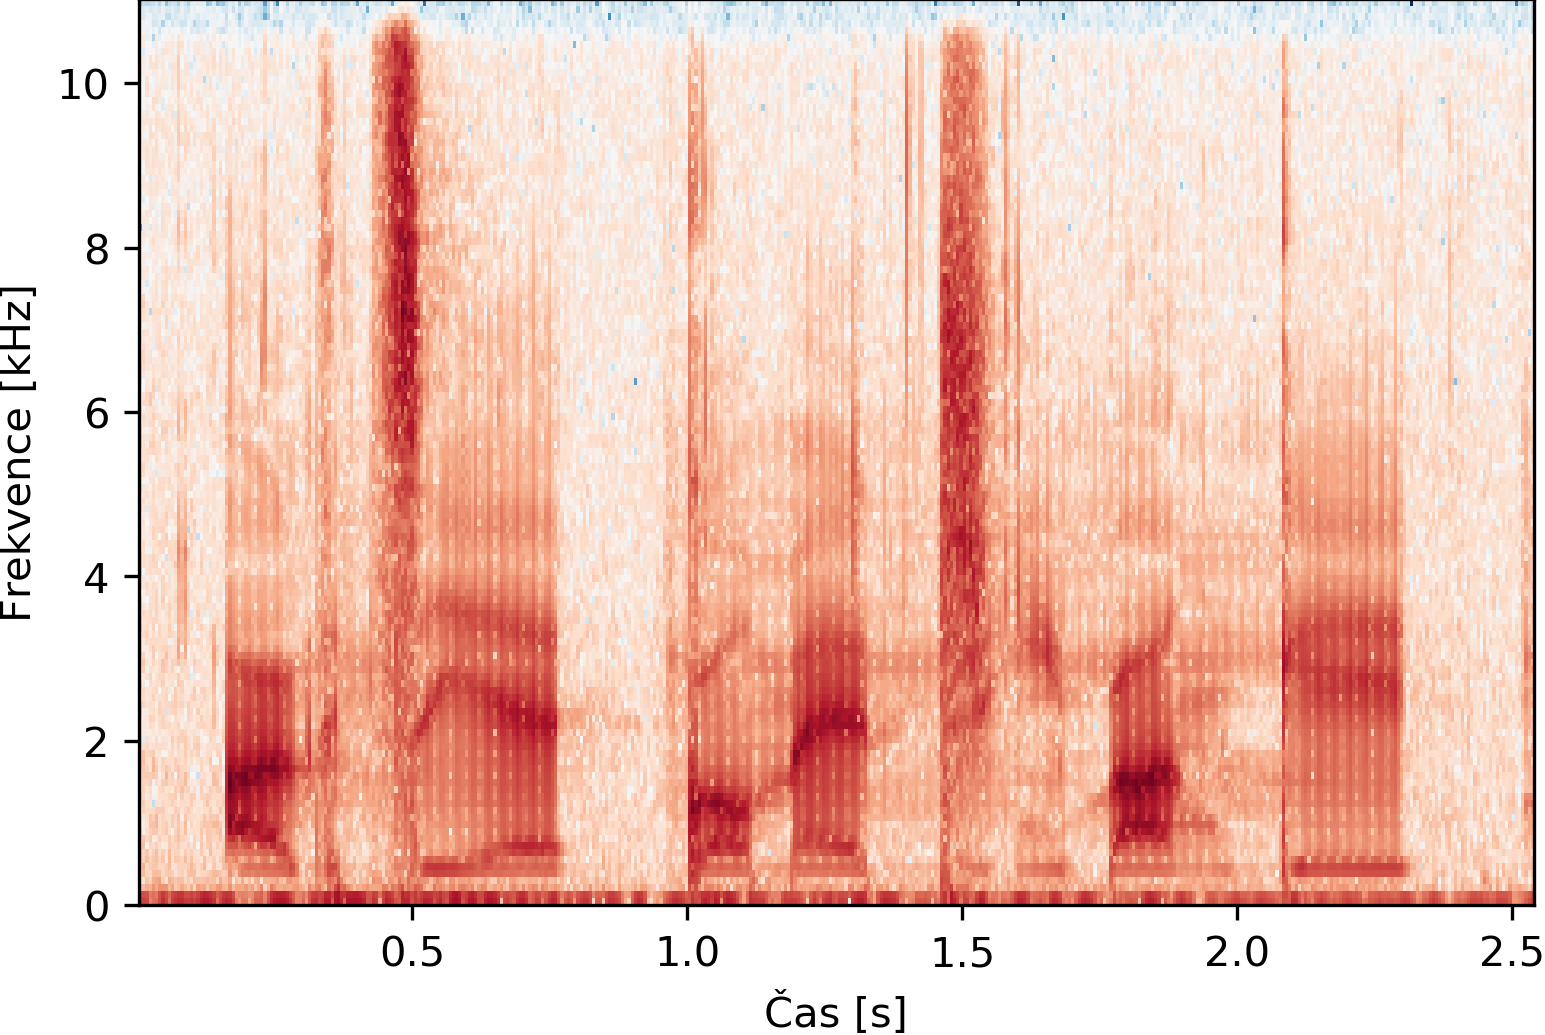
\includegraphics[width=\textwidth]{./ch4-experiments/img/spectrogram_el.png}
    \caption{EL řečník}
    \label{fig:experiments:analysis:spectrogram:el}
  \end{subfigure}
  \caption{Spektrogram promluvy \uv{Akcie Komerční banky} dvou řečníků.}
  \label{fig:experiments:analysis:spectrogram}
\end{figure}

Dalším způsobem jak porovnat řeč zdravého řečníka a tím s EL je pomocí analýzy jednotlivých fonémů. Na obr. \ref{fig:experiments:analysis:phonemes} jsou zobrazeny průběhy amplitudy v čase\footnote{Hodnoty času, na obr. \ref{fig:experiments:analysis:phonemes}, odpovídají časům výskytu v původní promluvě.} pro fonémy $/k/$, $/m/$ a $/\check{c}/$. V případě $/k/$ a $/m/$ (1. a 2. průběh) se jedná o okluzivy, kde v prvním případě se jedná o neznělou plozivu a druhém o znělou plozivu. Tyto fonémy obecně vznikají uzavřením vydechovaného proudu vzduchu, pomocí artikulačních orgánů, což se projeví jako krátká pauza (tzv. okluze). Po té následuje náhlé jednorázové překážky a únik nahromaděného vzduchu, tzv. exploze \cite{Psutka2006}. Takto popsáno to samozřejmě funguje u zdravého jedince, ale u EL řečníka jde principiálně o stejný mechanizmus. S tím rozdílem, že vzduch nepochází z plic, ale z hltanu. Dalším rozdílem je samozřejmě absence hlasivek.

\begin{figure}[htpb]
  \centering
  \begin{subfigure}[b]{0.42\textwidth}
    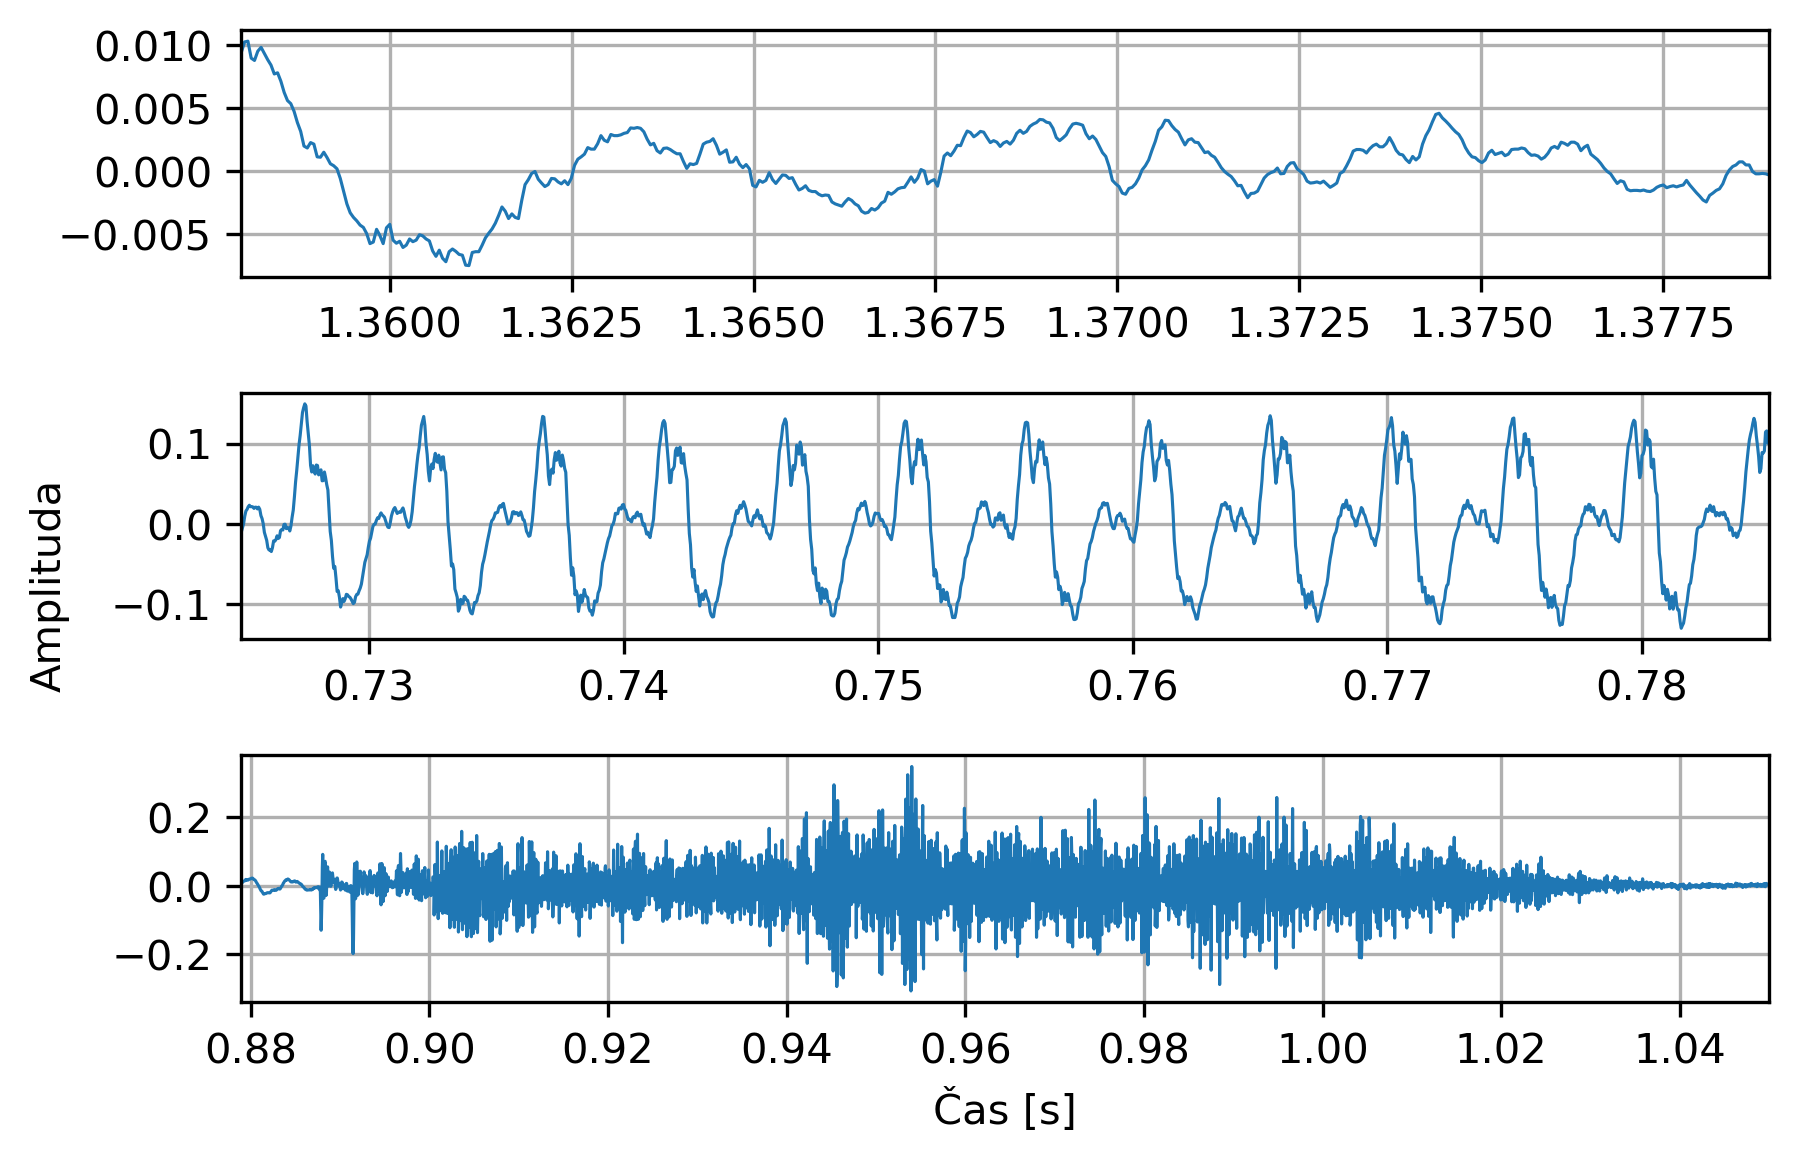
\includegraphics[width=\textwidth]{./ch4-experiments/img/phonemes_normal.png}
    \caption{Zdravý řečník}
    \label{fig:experiments:analysis:phonemes:normal}
  \end{subfigure}
  %
  \begin{subfigure}[b]{0.42\textwidth}
    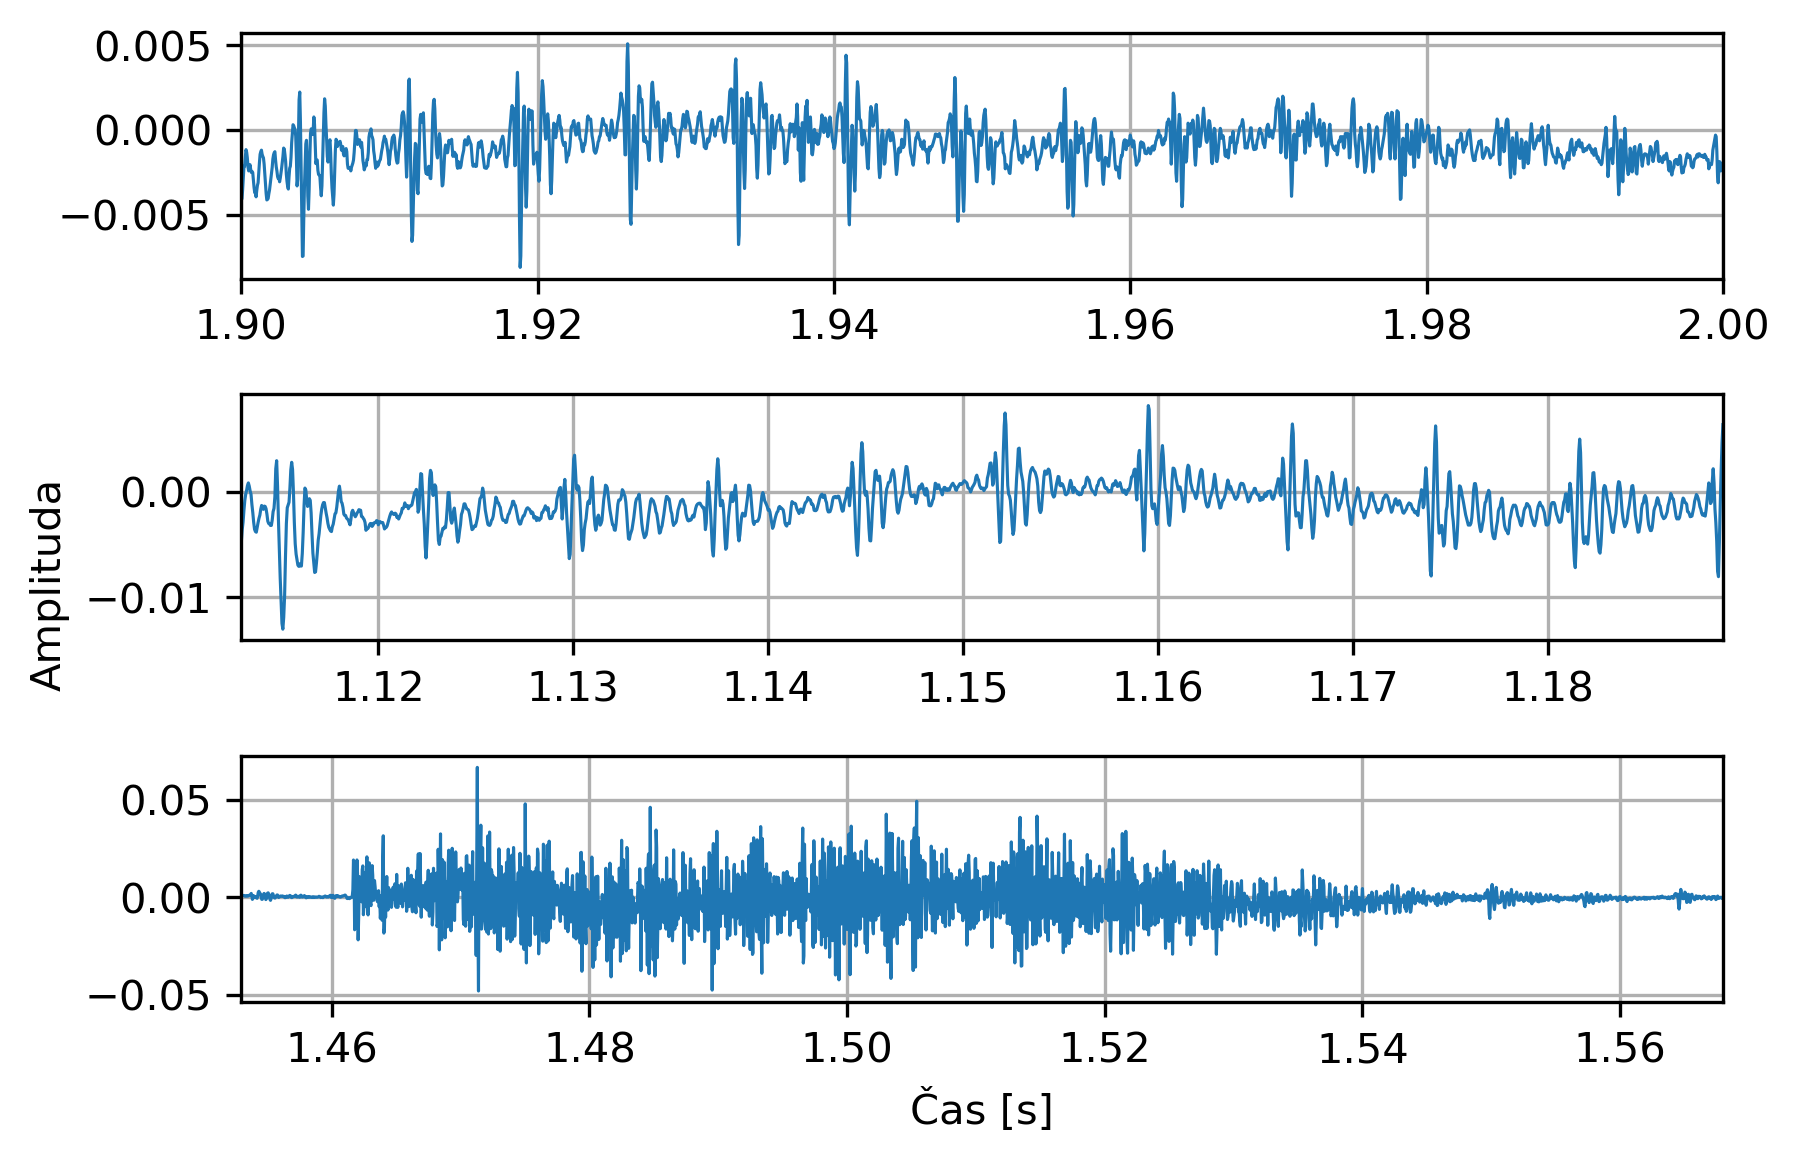
\includegraphics[width=\textwidth]{./ch4-experiments/img/phonemes_el.png}
    \caption{EL řečník}
    \label{fig:experiments:analysis:phonemes:el}
  \end{subfigure}
  \caption{Ukázky průběhů amplitudy pro fonémy $/k/$, $/m/$ a $/\check{c}/$.}
  \label{fig:experiments:analysis:phonemes}
\end{figure}

Foném $/k/$ představuje zástupce neznělých fonémů, ty se vyznačují tím, že do jejich produkce nezasahují hlasivky, které jsou v klidu. Zdrojem buzení je tedy šum. Pokud se podíváme na průběh amplitudy v čase u zdravého řečníka (obr. \ref{fig:experiments:analysis:phonemes:normal}), tak zde není vidět žádný periodický signál. Hlasivky jsou tedy opravdu v klidu. Oproti tomu u EL řečníka (obr. \ref{fig:experiments:analysis:phonemes:el}) je jasně patrné, že je zde přítomno aktivní buzení vytvořené EL. Na obr. \ref{fig:experiments:analysis:freq:k} je pak zobrazeno tzv. amplitudové spektrum, které znázorňuje vývoj amplitudy signálu ve frekcenci pro oba řečníky. V případě zdravého řečníka odpovídá vývoj očekávání tedy, že zde není žádná výrazná frekvence a také, že nedochází k výraznému útlumu. Přestože se v obou případech jedná o stejný foném, tak z časového i frekvešního průběhu amplitudy je zřejmé, že parametry signálu se u obou řečníku diametrálně liší.

\begin{figure}[hbpt]
  \centering
  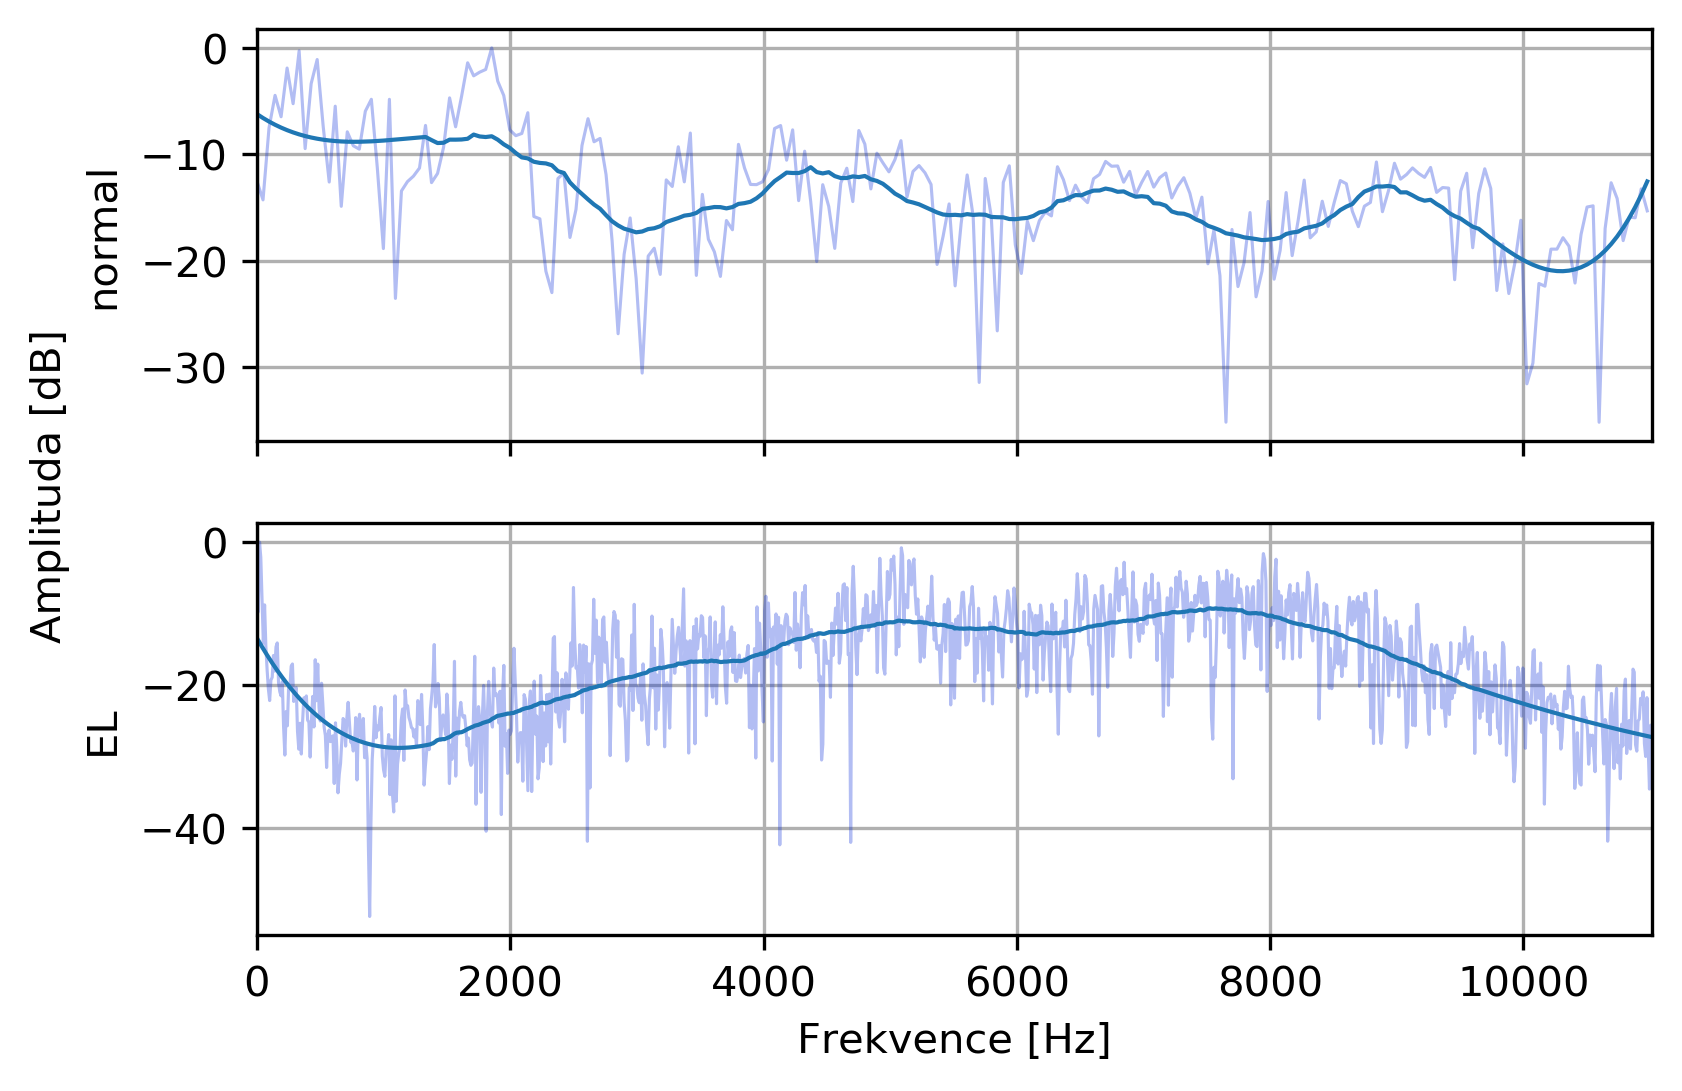
\includegraphics[width=0.9\textwidth]{./ch4-experiments/img/freq_analysis_(k).png}
  \caption{Vývoj amplitudy fonému $/k/$ ve frekvenci zdravého (horní) a EL (dolní) řečníka.}
  \label{fig:experiments:analysis:freq:k}
\end{figure}

Jako druhý ukázkový foném slouží $/m/$. Opět se jedná o plozivu, ale v tomto případě o znělou. U těchto fonémů hrají velký vliv hlasivky, protože jsou zdrojem buzení. Z obr. \ref{fig:experiments:analysis:phonemes:normal} je krásně zřetelné buzení ve formě perodického průběhu amplitudy. Narozdíl tomu, u EL řečníka (obr. \ref{fig:experiments:analysis:phonemes:el}) je také vidět periodický signál, ale úplně jiného průběhu. Svým způsoběm dost podobný tomu, který je zřetelný u fonému $/k/$. Rozdíl je zřetelný i ve frekvenční oblasti (obr. \ref{fig:experiments:analysis:freq:m}), kdy u EL řečnía nedochází útlumu ve střední oblasti frekvenčního spektra.

\begin{figure}[hbpt]
  \centering
  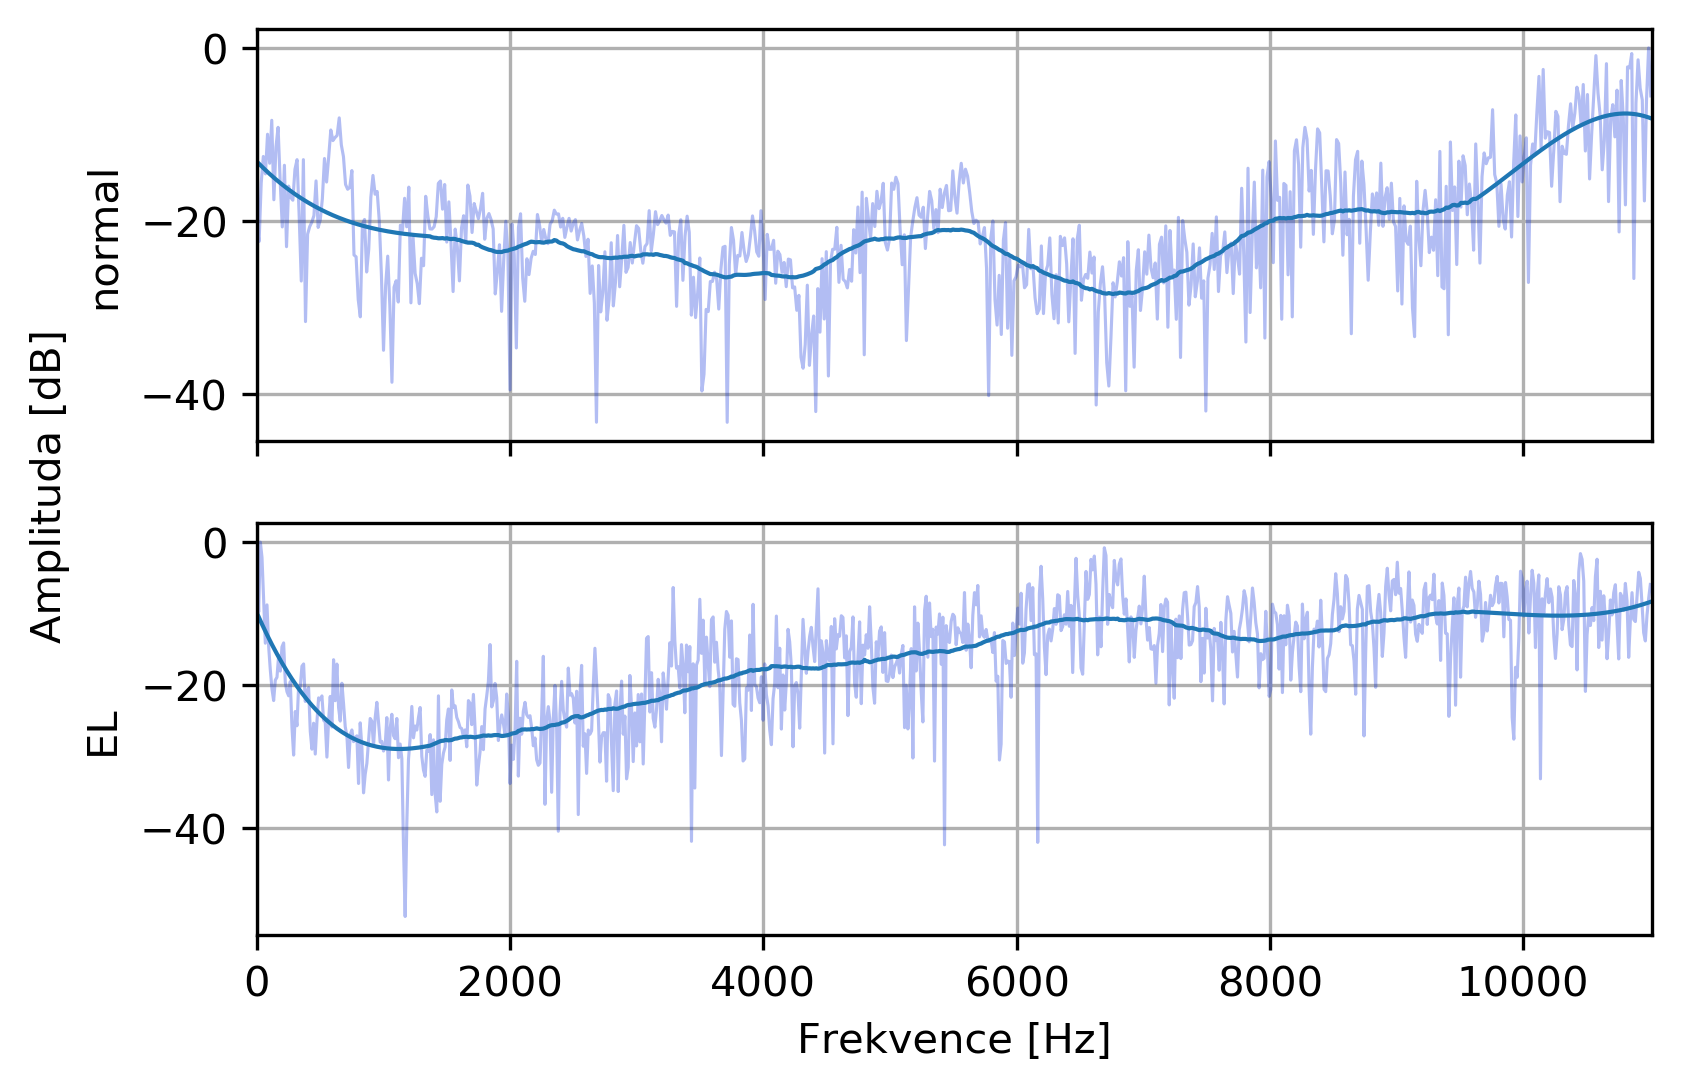
\includegraphics[width=0.9\textwidth]{./ch4-experiments/img/freq_analysis_(m).png}
  \caption{Vývoj amplitudy fonému $/m/$ ve frekvenci zdravého (horní) a EL (dolní) řečníka.}
  \label{fig:experiments:analysis:freq:m}
\end{figure}

Posledním úkázkovým fonémem je již zmiňované $/\check{c}/$. Jedná se o neznělý foném, který vzniká přiložením jazyku k zadní části horního patra. Tím je zadržen vzduch v dutině ústní a vzniká krátká pauza. Uvolněním pak dochází k explozi a vytvoření zvuku. Do produkce se nezapojují hlasivky a produkovaný zvuk by měl být dostatečně intenzivní, aby jej (v případě EL řečníka) tolik neovlivňoval EL. Tím pádem by měl být průběh signálu, u obou řečníků podobný, a to jak v časové, tak i ve frekvenční oblasti. Na obr. \ref{fig:experiments:analysis:phonemes} a \ref{fig:experiments:analysis:freq:c} je pak jasně vidět, že se jedná o platný předpoklad.

\begin{figure}[hbpt]
  \centering
  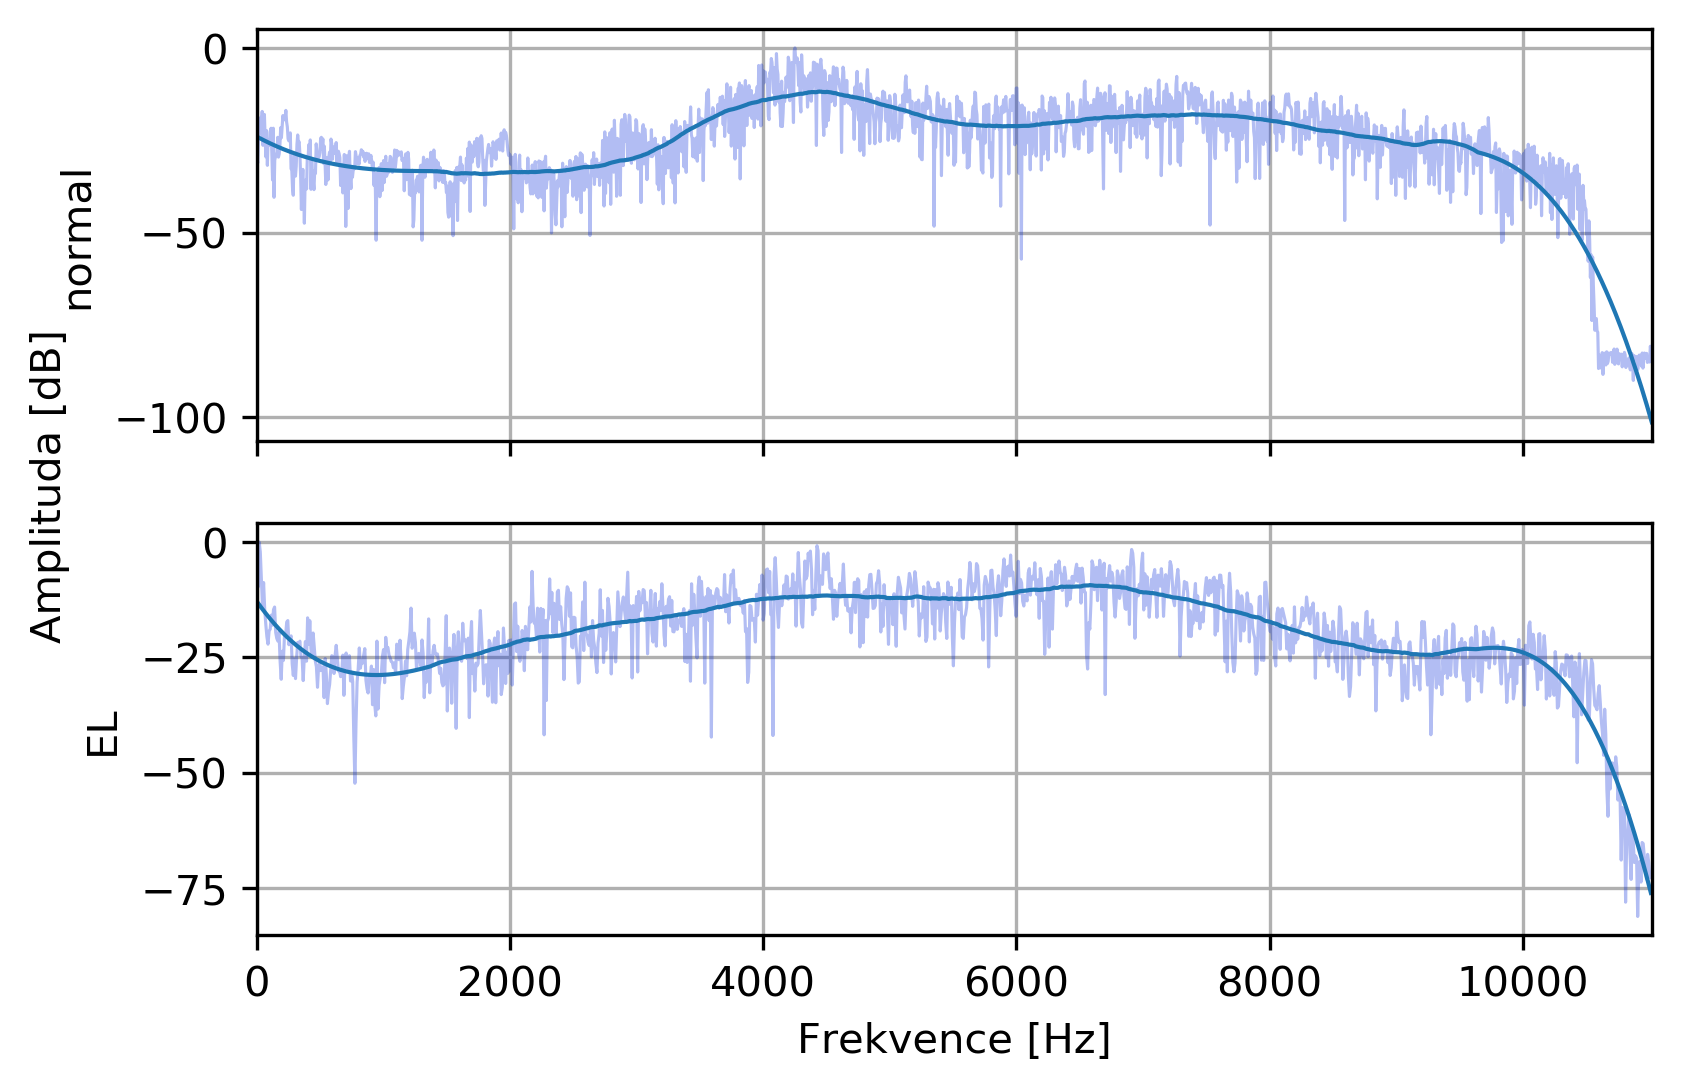
\includegraphics[width=0.9\textwidth]{./ch4-experiments/img/freq_analysis_(c).png}
  \caption{Vývoj amplitudy fonému $/\check{c}/$ ve frekvenci zdravého (horní) a EL (dolní) řečníka.}
  \label{fig:experiments:analysis:freq:c}
\end{figure}

Z doposud provedené analýzy plyne, že EL řeč je v mnoha charakteristikách odlišná od té produkované zdravým řečníkem. Zejména u porovnání ve frekvenční oblasti (obr. \ref{fig:experiments:analysis:freq:k} a \ref{fig:experiments:analysis:freq:m}) je to nejvíce patrné. Tento fakt nepochyně přispívá k tomu, že standardní obecné modely rozpoznávání řeči nedosahují takové přesnosti jako v případě bežné promluvy.

% \csvautotabular{./ch4-experiments/test.csv}

\subsection{Prvotní experimenty}
\label{chap:experiments:analysis:experiment}

Z provedené analýzy plyne, že EL data jsou od těch \uv{standardních} řečových relativně odlišná. Otazkou však je jak moc. Odpovědět může pomoci state-of-the-art obecný český ASR systém nezávislý na řečníkovi. V době psaní práce byl tento systém postaven na kombinaci neuronové sítě a skrytých makrovových modelů, tedy \textit{HMM-DNN}, více o těchto modelech v části \ref{chap:experiments:normalization}. K natrénováni modelu posloužil řečový korpus obsahující stovky hodin anotované řeči od velkého počtu řečníků. Pokud se jako vstup použily data ze získaného korpusu, tak byla dosažena přesnost slovní $18,49\ \%$\footnote{Pro potřeby této práce byl experiment zopakován v době psaní práce, protože od získání dat a první realizace tohoto experimentu uplynulo několik let a technologie pokročly. U původního experimentu byl výsledek obdobný.}. Toto číslo je vypočteno pomocí následujícího vzorce

\begin{equation}
  Acc = \frac{N - S - D - I}{N} * 100
  \label{eq:experiments:analysis:experiment:accuracy},
\end{equation}

\noindent kde $N$ je počet položek ve slovníku, $S$ je počet substitucí, $D$ je počet deletací a $I$ je počet inzercí.

Z dosaženého výsledku je patrné, že EL doména je diametrálně odlišná od bežné řeči, pro které jsou ASR systémy vytvářeny. Navíc, pokud se vezme v potaz náročnost získání potřebných dat pro natrénování obecného modelu, tak se jako jediná schůdná varianta jeví vytváření individuálních modelů pro každého řečníka. To znamená, že model je trénovaný pouze z dat odpovídající konkreténímu řečníkovi a často i účelu použití. K vytvoření takového modelu je zapotřebí řádově méně dat, při dosažení podobného výkonu. Stinnou stránkou je případná menší robustnost modelu. Čistě logicky tento model bude fungovat pouze s konkrétním řečníkem a ještě jen v situacích, které odpovídají trénovacím datům. U řečníků s EL může navíc hrát velký vliv samotný EL. Již při nahrávání se ukázalo, že jeho pozice může nepříznivě ovlivnit kvalitu řeči. Tento problém by však neměl významně ovlivňovat kvalitu modelu, protože tento fenomém je obsažen v datech. Co se však ukázalo jako potencionálně problematické, je stabilita parametrů produkované řeči v dlouhodobém časovém úseku. Více o tomto problému pak v části \ref{chap:experiments:normalization:quality}. K zodpovězení nejdůležitější otázky, jestli takový model vůbec může fungovat, stačí získaná data z první etapy nahrávání a ta obsahují řeč s relativně konzistentními parametry.

V rámci ověřování funkčnosti infividuálního modelu je vhodné zkusit různé varianty, aby se určili optimální parametry modelu. Hlavními uvažovanými hyperparametry je vzorkovací frekvence audio nahrávek a počet \textit{HMM} stavů. Originální pořízené nahrávky mají vzorkovací frekvenci rovnu $44,1\ kHz$, pro úlohu rozpoznávání je to zbytečně moc, protože nejvíce informace je obsažena ve frekvenčním pásmu do $4\ kHz$, vyšší frekcence a priory ovlivňují zabarvení hlasu apod. \cite{Psutka2006} Otázkou je jestli stačí vzorkovací frekvence rovna $8\ kHz$ nebo lépe $16\ kHz$, kde je přeci jen více informací. Počet stavý modelu pak ovliňuje množsví modelovaných trifónů. Čím více stavů, tím více je modelovaných trifónů. Stinnou stránkou pak je fakt, že čím více stavů, tím více  je potřeba trénovacích dat. Množina uvažovaných možností obsahuje $1024,\ 2048$ a $4096$ stavů. Jen pro vysvětlení je dobré zmínit, že \textit{HMM} stav představuje model jedné uvažované akustické jednotky (nebo skupiny jednotek s podobnými parametry). Počet stavů nám tedy říká, kolik takových jednotek model dokáže rozlišit. Čím více stavů, tím více jednotek (menších skupin) je modelováno. Teoreticky tak model s více stavy je lepší. Nicméně k natrénování jednotky je potřeba určité množství dat a tím pádem je pro model s vyšším počtem stavů logicky potřeba větší množství trénovacích dat. Samozřejmě fonetická sada neobsahuje $4096$ fonémů, neobsahuje ani $1024$ fonémů\footnote{Ve skutečnosti obsahuje 42 českých fonémů.}. U těchto modelů se pak používá nějaký druh \textit{n-gramové} reprezentace fonémů, nejčastěji pak trifóny.

Celkově je tak natrénováno $6$ modelů. K natrénování akustických modelů je použit HTK-Toolkitu v3.4., který je určen k vytváření \textit{HMM} modelů za pomocí k-means, Viterbiho a Baum-Welsch algoritmu.

Funkce ASR systému lze popsat rovnící

\begin{equation}
  \argmax_W p\left(W | O\right) = \argmax_W p\left(O | W\right) p\left(W\right),
\end{equation}

\noindent kde $O$ reprezentuje sekvenci akustických příznaků a $W$ výstupní sekvenci znaků\footnote{Znakem tu může být myšleno písmeno, případně slovo.}. $P\left(O | W\right)$ je pravděpodobnost generování korektní pozorované sekvence, tedy korektní k akustickému modelu ASR systému. Pravděpodobnost $P\left(W\right)$ je a priorní pravděpodobnost konkrétní sekvence znaků $W$, jinými slovy jazykový model. K získání výsledků je tedy potřeba mít i tento model. Ten však není níjak ovlivněn řečníkem (pouze doménou použití systému) a není jej třeba upravovat pro potřeby řečníka s EL. Cílem experimentu je ověření funkčnosti ASR a nalezení optimálních parametrů akustického modelu. Z tohoto důvodu je potřeba co nejvíce eliminovat vliv jazykového modelu na celkovém výkonu ASR systému. Jak bylo zmíněno, funkcí $p\left(W\right)$ je určení nejpravděpodobnější sekvnce znaků. Pravděpodobnostní rozložení je získáno z velkého množství trénovacích textů. Toto natrénované rozložení by však velmi ovlivnilo výsledky experimentů, a proto je použít zerogramový monofónový model. Ten se vyznačuje tím, že všechny prvky slovníku mají stejnou pravděpodobnost rovnu $P(w_n) = \frac{1}{N}$, kde $N$ je počet položek ve slovníku. Monofónový model je navíc zvolen z toho důbodu, že fonetická sada je známa a obsahuje malý počet jednotek. Z pohledu jazykového modelu má libovolný výstup z akustického modelu stejnou pravděpodobnost výskytu a tím pádem se jazykový model nijak nepřispívá k celkové kvalitě ASR systému.

Tab. \ref{tab:experiments:analysis:experiment:gmm} znázorňuje dosažené výsledky. Hlavním poznatkem je fakt, že individuální ASR systém může fungovat. Pokud dosažené výsledky porovnáme s výsledky v \textbf{TBD}, tak je vidět rapidní nárůst výkonu, \todo{Doplnit}{$XX.XX$} obecného modelu oproti $78,63\ \%$ u nejhoršího individuálního modelu. Ze získaných dat je pak jasně patrné, že použití vzorkovací frekvence rovné $16\ kHz$ s sebou nese významné zlepšení přesnosti o $1,41\ \%$ absolutně, tedy téměř $7\ \%$ relativně. V dodatečných experimentech se pak ukázalo, že použití vyšší frekvence již přinese žádné nebo zanedbatelné zlepšení.

Počet stavů již pak nehraje, tak zásádní roli na kvalitu akustického modelu jako vzorkovací frekvence. Z testované množiny maximálního počtu stavů dosáhl nejlepšího výsledku model, který měl maximálně $4096$ stavů, nicméne oproti modelu s $1024$ stavy je nárůst přesnosti pouze $0,4\ \%$ absolutně v případě $16\ kHz$ modelů, což není tak významné. Logicky se nabízí otázka, proč nezkusit ještě více stavů? Odpověď na tuto otázku se skrývá ve skutečném počtu stavů modelu s maximálním počtem $4096$ stavů. Slovíčko \uv{maximálním} je zde podstatné. Algoritmus trénování akustického modelu se snaží rozdistribuovat všechny možné akustické jednotky (v tomto případě trifóny) do maximálního počtu stavů. Pokud je méně stavů než jednotek, tak dochází k určité formě shlukování (často může posloužit \textit{k-means} algoritmus). Pokud je dostatek dat k natrénování konkrétního shluku, je tento shluk použit, pokud není dostatečné množství dat, je tento shluk spojen s jiným, který je svými parametry nejblíže. Tím pádem se mohou stát dvě věci. Je k dizpozici dostatek dat k natrénování maximálního počtu stavů a nebo není dostatek dat k natrénování maximálního počtu stavů. U modelu s maximálním počtem $4096$ stavů je skutečný počet stavů přibližně $3200$, i kdyby se natrénoval model s $8192$, tak by se tato hodnota nezměnila. Pro doplnění, monofónový akustický model dosáhl přesnosti $54,49\ \%$ pro $8\ kHz$ a $62,30\ \%$ pro $16\ kHz$.

\begin{table}[htpb]
  \centering
  \def\arraystretch{1.5}
  \pgfplotstabletypeset[
    col sep=semicolon,
    string type,
    columns/model/.style={column name=Model, column type={|c}},
    columns/8k/.style={column name=8 kHz $[\%]$, column type={|r}},
    columns/16k/.style={column name=16 kHz $[\%]$, column type={|r|}},
    every head row/.style={before row={
      \hline
      & \multicolumn{2}{c|}{Accuracy} \\
    },after row=\hline},
    every last row/.style={after row=\hline},
  ]{./ch4-experiments/tabs/01-frequency.csv}
  \caption{Vliv frekvence na kvalitu modelu.}
  \label{tab:experiments:analysis:experiment:gmm}
\end{table}

Jelikož tento experiment byl realizován na přelomu let $2013$ a $2014$, kdy ještě $ASR$ modelům dominovaly \textit{HMM-GMM} modely, byl později zopakován s \textit{HMM-DNN} modely, které dosahují ještě vyšších přesností. Více o \textit{HMM-DNN} v části \ref{chap:experiments:normalization:corpus}. Výsledky těchto modelů jsou v tab. \ref{tab:experiments:analysis:experiment:dnn}, z nich je vidět, že i v této oblasti neuronové sítě jasně dominují.

\begin{table}[htpb]
  \centering
  \def\arraystretch{1.5}
  \pgfplotstabletypeset[
    col sep=semicolon,
    string type,
    columns/model/.style={column name=Model, column type={|c}},
    columns/8k/.style={column name=8 kHz $[\%]$, column type={|r}},
    columns/16k/.style={column name=16 kHz $[\%]$, column type={|r|}},
    every head row/.style={before row={
      \hline
      & \multicolumn{2}{c|}{Accuracy} \\
    },after row=\hline},
    every last row/.style={after row=\hline},
  ]{./ch4-experiments/tabs/01-frequency_dnn.csv}
  \caption{Vliv frekvence na kvalitu modelu využívajícího \textit{DNN} }
  \label{tab:experiments:analysis:experiment:dnn}
\end{table}

\subsection{Redukce fonetické sady}
\label{chap:experiments:analysis:reduction}

Při používání EL je přístroj v průběhu promluvy permanentně zapnutý a to i v případě neznělých fonémů. Jejich rozdílný průběh je patrný na obr. \ref{fig:experiments:analysis:phonemes}. Nabízí se tak předpoklad, že všechny neznělé fonémy mají podobu znělých fonémů a tím pádem je možné redukovat fonetickou sadu. Teoreticky, pokud jsou všechny neznělé fonémy produkovány jako znělé, a je redukována fonetická sada, tak je snížena perplexita modelu a ten by měl být schopen pracovat s vyšší přesností.

K ověření tohoto předpokladu je potřeba experimentálního ověření. Myšlenka experimentu je jednoduchá. Je potřeba natrénovat několik modelů lišících se pouze tím, jaký fonetický pár (viz tab. \ref{tab:experiments:analysis:reduction:pairs}) byl použit pro redukci fonetické sady. V rámci experimentu jsou uvažovány tyto případy:

\begin{itemize}
  \item \textit{Baseline} - standardní model s plnou fonetickou sadou.
  \item $/f/ \rightarrow /v/$ - foném $/f/$ je nahrazen fonémem $/v/$.
  \item $/k/ \rightarrow /g/$ - foném $/k/$ je nahrazen fonémem $/g/$.
  \item $/s/+/\check{s}/ \rightarrow /z/+/\check{z}/$ - foném $/s/$ $\left(/\check{s}/\right)$ je nahrazen fonémem $/z/$ $\left(/\check{z}/\right)$.
  \item $/t/+/\text{\textit{ť}}/ \rightarrow /d/+/\text{\textit{ď}}/$ - foném $/t/$ $\left(/\text{\textit{ť}}/\right)$ je nahrazen fonémem $/d/$ $\left(/\text{\textit{ď}}/\right)$.
  \item \textit{Náhrada všech} - všechny neznělé fonémy jsou nahrazeny znělým ekvivalentem.
\end{itemize}

\begin{table}[htpb]
  \centering
  \def\arraystretch{1.5}
  \pgfplotstabletypeset[
    col sep=comma,
    string type,
    columns/unvoiced/.style={column name=Neznělé fonémy, column type={|c}},
    columns/voiced/.style={column name=Znělé fonémy, column type={|c|}},
    every head row/.style={before row={
      \hline
    },after row=\hline},
    every last row/.style={after row=\hline},
  ]{./ch4-experiments/tabs/phonemes_pairs.csv}
  \caption{Korespondující páry fonémů.}
  \label{tab:experiments:analysis:reduction:pairs}
\end{table}

\noindent Pro porovnání jsou stejné modely vytvořeny i pro zdravého řečníka. U něj by, při libovolné redukci fonetické sady, mělo dojít ke zhoršení oproti \textit{baseline} modelu.

K natrénování akustických modelů byly použity korpusy čítající 5000 vět\footnote{Pro oba řečníky jsou použity stejné věty pocházející z databáze popsané v \cite{Radova2000}.}, což představuje více než 10 hodin řeči pro každého řečníka. Akustická data byla parametrizována pomocí MFCC s 26 filtry a 12 kepstrálními koeficienty a energií. Dále vektor parametrů obsahuje delta a delta-delta příznaky. To dohromady dává vektor 40 příznaků pro každých 10 ms náhrávky \cite{Psutka2007}.

V rámci experimentu byly otestovány dva přístupy vzájemně se lišící řečovou jednotkou. V prvním případě se jednalo o monofónový akustický model a v druhém trifónový. U obou přístupů je řečová jednotka reprezentována třístavovým \textit{HMM} modelem se spojitou výstupní pravděpodobnostní funkcí pro každý stav. Jelikož je pro češtinu množství trifónů opravdu velké, jsou využity fonetické rozhodovací stromy pro určení trifónů a korespujících stavů. Jednoduše řečeno jsou vytvořeny shluky trifónů, protože většinou není k dispozici dostatek dat pro natrénování všech variant trifónů. Pro určení optimálních parametrů modelu pro EL byly použity znalosti z části \ref{chap:experiments:analysis:experiment}. Pro zdravého řečníka je pro každou část experimentu vytvořeno několik modelů lišící se počtem stavů a gaussovkých směsí. Všechny akustické modely jsou natrénovány pomocí HTK-Toolkitu v3.4. Celkem bylo vytvořeno 24 akustických modelů, 12 pro EL řečníka (6 monofónových a 6 trifónových) a 12 pro zdravého řečníka.

Pro otestování modelů byla vytvořena testovací sada čítající 500 vět náhodně vybraných z původních korpusů (pro oba řečníky stejná). Testovací sada tak představuje přibližně 1 hodinu řeči pro každého řečníka. Pro fungování ASR systému je potřeba, kromě akustického, i jazykový model. Ten určuje pravděpodobnost písmene/slova na základě předchozích pozorování. V rámci tohoto experimentu jsou uvažovány dva jazykové modely

\begin{enumerate}
  \item \textit{zerogramový jazykový model} - v tomto případě mají všechna slova v modelu stejnou pravděpodobnost $P_r(w_n|w_1,\dots,w_{n-1}) = \frac{1}{N}$, kde $N$ je počet slov ve slovníku. V tomto případě $N = 2885$, jinýmy slovy perplexita modelu je $2885$. Testovací slovník je vytvořen z testovací sady, model tedy naobsahuje OOV\footnote{Out-of-vocabulary (OOV) - slova, která nejsou obsažena ve slovníku jazykového modelu.}.
  \item \textit{trigramový jazykový model} - u tohoto modelu odpovídá pravděpodobnost následujícího slova $P_r(w_n|w_1,\dots,w_{n-1})~=~p(w_n|w_{n-2}, w_{n-1})$. K získání $p(w_n|w_{n-2}, w_{n-1})$ posloužil SRILM Toolkit s Kneser-Ney vyhlazováním\footnote{Vyhlazování slouží k vyřešení problému s OOV, kdy trénovací data neobsahovala OOV, a proto není k dispozici $p(w_n|w_{n-2}, w_{n-1})$.} \cite{Stolcke2002}, které se podle \cite{Prazak2008} ukázalo jako optimální pro tyto typy modelů. Jako trénovací data byly použity texty z novinových článků, webových stránek a přepisů televizních pořadů. Celkem model obsahuje 360K nejvíce frekventovaných slov. OOV bylo $3,8 \%$ a perplexita $3380$.
\end{enumerate}

\noindent V kombinaci s vytvořenými akustickými modely to představuje 4 dílčí experimenty. Jen pro doplnění je nutné poznamenat, že přesnost modelů je vyhodnocována na slovech.

Tab. \ref{tab:experiments:analysis:reduction:01} a \ref{tab:experiments:analysis:reduction:02} zobrazují výsledky\footnote{V tomto případě jsou výsledky udávány ve formě přesnosti, protože se zde využívá HTK oproti Kaldi v ostatních experimentech.} pro monofónový akustický model a zerogramový jazykový model, resp. trigramový jazykový model. V obou případech je vidět očekávané chování přesnosti modelu u zdravého řečníka. Ke konečné podobě fonetické sady se dospělo po dlouholetém výzkumu a počet fonémů je tak optimální. Redukcí fonetické sady je omezena komplexita modelu a tím pádem dochází ke zhoršení přesnosti. Překvapující může být horší výsledky u zdravého řečníka v tab. \ref{tab:experiments:analysis:reduction:02}. Toto chování může být vysvětleno vyšší perplexitou trigramového jazykového modelu v kombinaci s relativně jednoduchým monofónovým akustickým modelem.

U EL řečníka je vidět dílčí zlepšení u 2 modelů (tab. \ref{tab:experiments:analysis:reduction:01}), resp. 1 modelu v případě trigramového modelu (tab. \ref{tab:experiments:analysis:reduction:02}). Ve většině případech však redukce fonetické sady vedla ke zhoršení přesnoti. U EL řečníka došlo ke zlepšení při použití trigramového jazykového modelu, to nasvědčuje tomu, že monofónový akustický model není úplně ideální pro odhad sekvence fonémů.

\begin{table}[htpb]
  \centering
  \def\arraystretch{1.5}
  \pgfplotstabletypeset[
    col sep=semicolon,
    string type,
    columns/model/.style={column name=Model, column type={|c}},
    columns/normal/.style={column name=Zdravý $[\%]$, column type={|r}},
    columns/el/.style={column name=EL $[\%]$, column type={|r|}},
    every head row/.style={before row={
      \hline
    },after row=\hline},
    every last row/.style={after row=\hline},
  ]{./ch4-experiments/tabs/reduction_01.csv}
  \caption{Vliv redukce fonetické sady na přesnost ASR systému s monofóním akustickým a zerogramovým jazykovým modelem pro zdravého a EL řečníka.}
  \label{tab:experiments:analysis:reduction:01}
\end{table}

\begin{table}[htpb]
  \centering
  \def\arraystretch{1.5}
  \pgfplotstabletypeset[
    col sep=semicolon,
    string type,
    columns/model/.style={column name=Model, column type={|c}},
    columns/normal/.style={column name=Zdravý $[\%]$, column type={|r}},
    columns/el/.style={column name=EL $[\%]$, column type={|r|}},
    every head row/.style={before row={
      \hline
    },after row=\hline},
    every last row/.style={after row=\hline},
  ]{./ch4-experiments/tabs/reduction_02.csv}
  \caption{Vliv redukce fonetické sady na přesnost ASR systému s monofóním akustickým a trigramovým jazykovým modelem obsahujícím 360k slov pro zdravého a EL řečníka.}
  \label{tab:experiments:analysis:reduction:02}
\end{table}

V tab. \ref{tab:experiments:analysis:reduction:03} a \ref{tab:experiments:analysis:reduction:04} jsou pak vypsány výsledky pro trifónový akustický model se zerogramovým resp. trigramovým jazykovým modelem. Stejně jako u předchozích dvou experimentů, tak i zde je vidět, že redukce fonetické sady vede u zdravého řečníka vždy ke zhoršní přesnosti modelu. Také je tu možné vydedukovat, že trifónový akustický model dosahuje výrazně lepších výsledků než monofónní model. Zhoršení u EL řečníka v tab. \ref{tab:experiments:analysis:reduction:03} je s největší pravděpodobností způsobeno fonetickými stromy, protože není dostatek dat pro všechny možné varianty trifónů. Tím pádem model pro určité trifóny vrací špatné sekvence znaků. Zerogramového jazykový model to pak nedokáže zachránit, protože všechny slova mají stejnou pravděpodobnost $P_r(w_n|w_1,\dots,w_{n-1}) = \frac{1}{2885}$. Tím pádem může dojít k rozpoznávání špatného slova a nižší celkové přesnosti. Tuto domněnku potvrzuje rapidní zlepšení v případě trigramového jazykového modelu (tab. \ref{tab:experiments:analysis:reduction:04}), kde již jazykový model významně přispívá k přesnosti modelu.

U obou experimentů s trifónovým jazykovým modelem došlo ke zlepšení u dvou modelů (tab. \ref{tab:experiments:analysis:reduction:03} a \ref{tab:experiments:analysis:reduction:04}), ale stejně jako v případě monofónového modelu vedla ve většině případů redukce fonetické sady ke zhoršení.

\begin{table}[htpb]
  \centering
  \def\arraystretch{1.5}
  \pgfplotstabletypeset[
    col sep=semicolon,
    string type,
    columns/model/.style={column name=Model, column type={|c}},
    columns/normal/.style={column name=Zdravý $[\%]$, column type={|r}},
    columns/el/.style={column name=EL $[\%]$, column type={|r|}},
    every head row/.style={before row={
      \hline
    },after row=\hline},
    every last row/.style={after row=\hline},
  ]{./ch4-experiments/tabs/reduction_03.csv}
  \caption{Vliv redukce fonetické sady na přesnost ASR systému s trifónovým akustickým a zerogramovým jazykovým modelem pro zdravého a EL řečníka.}
  \label{tab:experiments:analysis:reduction:03}
\end{table}

\begin{table}[htpb]
  \centering
  \def\arraystretch{1.5}
  \pgfplotstabletypeset[
    col sep=semicolon,
    string type,
    columns/model/.style={column name=Model, column type={|c}},
    columns/normal/.style={column name=Zdravý $[\%]$, column type={|r}},
    columns/el/.style={column name=EL $[\%]$, column type={|r|}},
    every head row/.style={before row={
      \hline
    },after row=\hline},
    every last row/.style={after row=\hline},
  ]{./ch4-experiments/tabs/reduction_04.csv}
  \caption{Vliv redukce fonetické sady na přesnost ASR systému s trifónovým akustickým a trigramovým jazykovým modelem s 360k slov pro zdravého a EL řečníka.}
  \label{tab:experiments:analysis:reduction:04}
\end{table}

Ze získaných výsledků je možné usoudit, že redukce fonetické sady může vést ke zlepšení přesnosti. Nicméně předpoklad, že všechny neznělé fonémy jsou shodné se svými znělými ekvivalenty se nepotvrdila. Zároveň není možné úplně říci, že je možné, např. dvojici $/s/$ a $/\check{s}/$, za každých okolností převést na znělou variantu a dosáhnout tím lepších výsledků. Při hlubší analýze výsledků se ukázalo, že velmi záleží na kontextu daného fónemu, protože jeho podubu velmi ovlivňují fonémy v bezprostředním okolí. Řeč představuje spojitou formu signálu a při vyslovování různých slov obsahujícím stejný foném s odlišným okolím dochází i třeba k odchylkám v artikulaci, např. \textit{hrad} vs. \textit{hod}. Toto pozorování ověřil i dodatečný experiment, ve kterém se u náhrady $/s/$ za $/z/$ vynechal trifón \textit{b-s+t}, který je nápříklad ve slově \textit{obstát}. Díky vynechání tohoto trifónu byla výsledná nejlepší přesnost u trifónového akustického modelu $83,39\ \%$ v případě zerogramového jazykového modelu a $88,37\ \%$ v případě trigramového modelu. Přestože se jedná o marginální zlepšení, tak ho bylo docíleno jedním trifónem. Nicméně určení toho jaké trifóny vynechat z nahrazování není triviání úloha.

Zajímavý je také rozdíl mezi přesností modelu pro zdravého a EL řečníka. Přestože se v obou případech jedná o individuální modely šité \uv{na míru} řečníkovi, tak průměrný rozdíl je $6,24\ \%$ absolutně a $40,38\ \%$ relativně. To značí, že je potřeba se zabývat myšlenkou jak upravit akustický model, aby dosahoval lepších výsledků a v ideálním případě dosahoval podobných výkonů jako modely pro zdravé řečníky.

Naopak očekávaným výsledkem bylo zhoršená přesnosti pro zdravého řečníka ve všech případech redukce fonetické sady. Dále se potvrdilo, že komplexnější trifónový model dosahuje ve většině případů lepších výsledků. To je nepochybně způsobeno tím, že každý foném máme modelován pomocí více \textit{HMM} stavů, protože se bere v potaz i jeho okolí, kdežto pro monofónový model nikoli.
